\section{Risultati}

Come preannunciato nella sezione introduttiva, l'obiettivo principale dello studio è quello di confrontare tra loro diversi modelli di \texttt{dac}, ognuno dei quali caratterizzato da una differente modellazione della rete neurale che implementa in meccanismo di apprendimento del controller, e verificare come il meccanismo di apprendimento è influenzato dalla differente configurazione sensoriale (virtuale \ref{lab:ANN}) che li caratterizza.

I dati di seguito riportati sono relativi all'addestramento e test dei vari modelli di robot realizzati. Per ognuno di essi si sono esplorati diversi (sotto) spazi di valori dei parametri che guidano il comportamento e l'apprendimento dell'agente.

Al fine di concentrarsi ai soli parametri non banali, si è deciso di lasciare fisse le soglie di attivazione $\tau_{Motor}=1.0$ e $\tau_{Reverse}=2.0$. Queste soglie risultano banali in quanto:

\begin{itemize}
    \item Ogni neurone del layer di Collisione produce solo valori di output \texttt{\{0, 1\}}
    
    \item Si vuole modulare la velocità delle ruote in base al numero di neuroni attivi ($o_i=1.0$) su un determinato lato
    
    \item Si vuole invertire il senso di marcia se e solo se entrambi i neuroni frontali sono attivi ($o_0=1.0 \wedge o_7=1.0$)
\end{itemize}

Di conseguenza, nel caso di $\tau_{Motor}=1.0$, si ha un comportamento equivalente a $a_j = h_j$, che porta ad avere un incremento della velocità in una delle ruote proporzionale al numero di neuroni attivi collegati al neurone che soprassiede tale ruota. Nel caso di $\tau_{Reverse}$, la soglia dovrà essere $\tau_{Reverse}=N_{Reverse_j}$, nel nostro caso $N_{Reverse_j}=2.0$, se vogliamo che questi si attivi se e solo se tutti i neuroni ad esso connessi siano attivi.\\
\hfill\break
Dunque i parametri della quale si è deciso di esplorare lo spazio delle soluzioni sono:

\begin{itemize}
    \item $\eta$ -- Learning Rate
    \item $\epsilon$ -- Forget Rate
    \item $\tau_{Collision}$ -- Collision Threshold
\end{itemize}

\newpage

\subsection{Addestramento e Test}
% Elenca per ogni modello generato quali sono i range di parametri esplorati
% e perchè sono stati scelti questi parametri

Ogni modello descritto in \ref{marker:dacmodels} è stato addestrato, per ogni parametro, su un range di valori che fosse contenuto ma risultasse significativo, ovvero che contenesse con buona probabilità una o più configurazioni di parametri che avrebbero portato l'agente ad un corretto o almeno parziale apprendimento del comportamento. Questo range è stato definito in maniera totalmente empirica: prima dell'esecuzione dell'addestramento in modalità "batch" sono state avviate manualmente una serie di simulazioni di addestramento al fine di individuare un paio di esempi funzionanti, attorno alla quale è stato definito (grossolanamente) un range di valori per ogni parametro.

Sebbene in \cite{verschure1992distributed} fossero indicati alcuni di questi parametri con precisione ($\eta = 0.1, \epsilon = 0.5, \tau_{Collision} = 0.5$), test manuali effettuati con tali parametri non hanno portato risultati significativi. Ci si è dunque serviti di tali elementi solo come spunto iniziale di studio dello spazio dei parametri.

Nello specifico ogni modello ogni modello è stato addestrato con i seguenti range di parametri:

\begin{itemize}
    \item \texttt{dacv2} $\begin{cases}
            \eta \in [0.035, 0.065] & \text{with $\delta_{step}=0.005$}\\
            \epsilon \in [0.6, 0.9] & \text{with $\delta_{step}=0.05$}\\
            \tau_{Collision} \in [0.65, 0.95] & \text{with $\delta_{step}=0.05$}\\
    \end{cases}$
  
    \item \texttt{dacv3} $\begin{cases}
            \eta \in [0.065, 0.095] & \text{with $\delta_{step}=0.005$}\\
            \epsilon \in [0.6, 0.9] & \text{with $\delta_{step}=0.05$}\\
            \tau_{Collision} \in [0.55, 0.95] & \text{with $\delta_{step}=0.05$}\\
    \end{cases}$
    
    \item \texttt{dacv4} $\begin{cases}
            \eta \in [0.065, 0.1] & \text{with $\delta_{step}=0.005$}\\
            \epsilon \in [0.6, 0.9] & \text{with $\delta_{step}=0.05$}\\
            \tau_{Collision} \in [0.65, 0.95] & \text{with $\delta_{step}=0.05$}\\
    \end{cases}$
\end{itemize}
\hfill\break
% Specifica il tempo di apprendimento assegnato ad ogni agente

Sia in fase di addestramento che in fase di test si è lasciato l'agente ad apprendere o girovagare all'interno dell'arena per un tempo pari a 2h (del simulatore).

% Mostra immagine Arena Training
% Mostra immagine Arena Test
\begin{figure}[H]
    \centering
    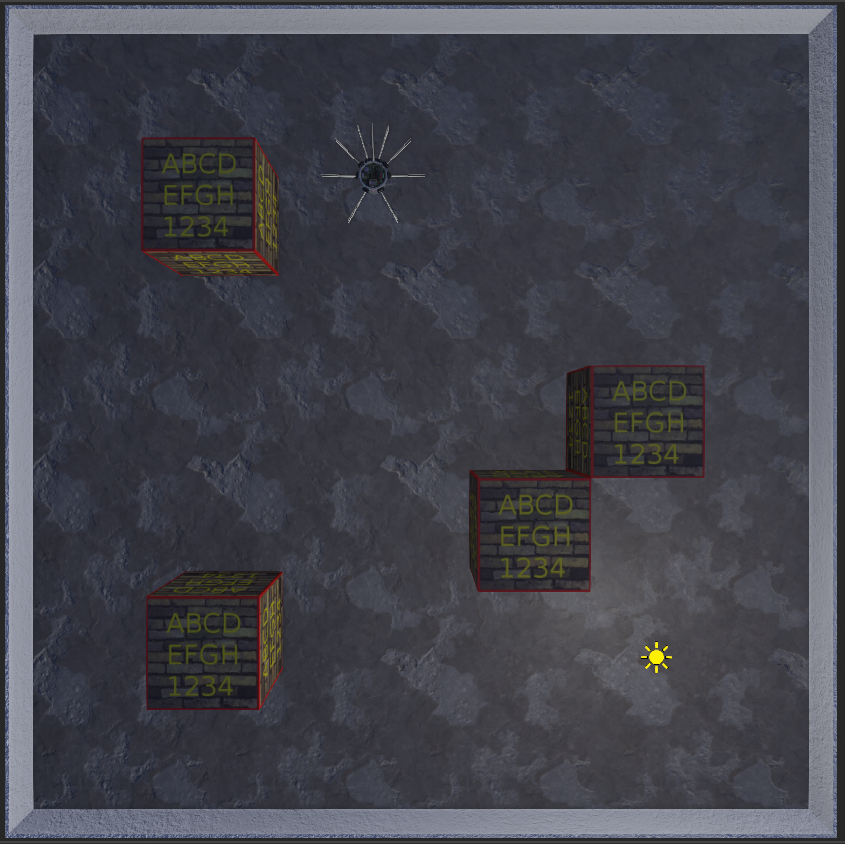
\includegraphics[scale=0.32,valign=t]{figures/train_arena.png}
    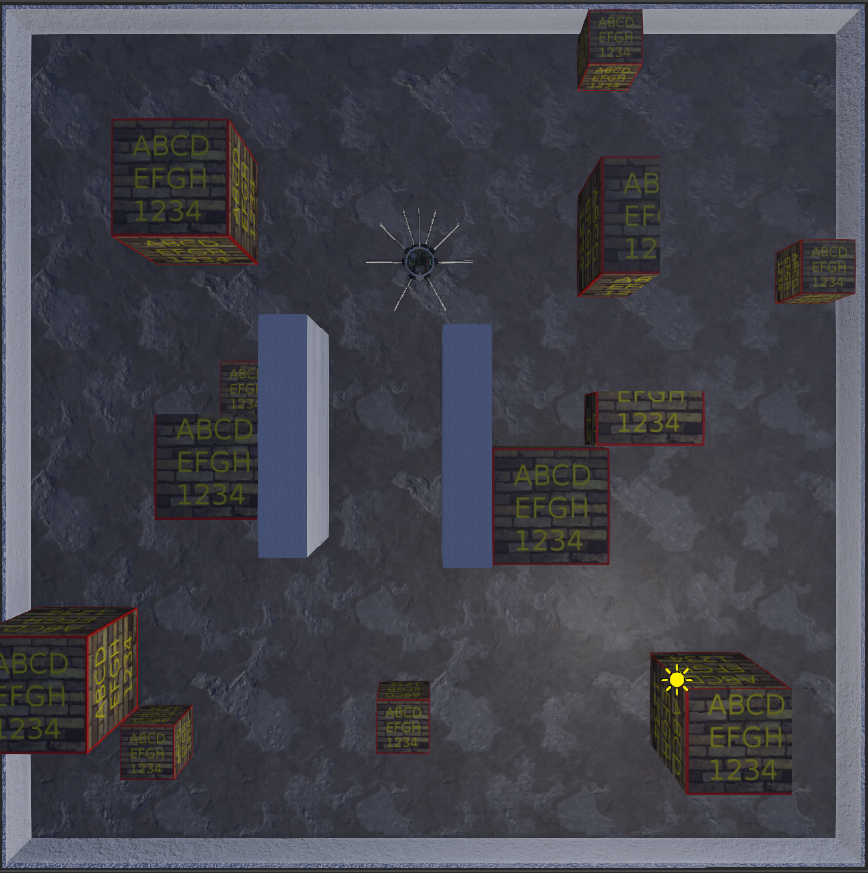
\includegraphics[scale=0.309,valign=t]{figures/test_arena.png}
    \caption{L'arena di addestramento (a sinistra) è stata realizzata volutamente semplice al fine di consentire all'agente di "apprendere" solo le situazioni di base, lasciando all'arena di test (visibile nell'immagine a destra) di verificare se il robot fosse in grado di generalizzare il comportamento appreso e in caso presentare comportamenti emergenti per configurazioni novelle degli ostacoli.}
    \label{fig:TrainArena}
\end{figure}

\subsection{Performance}

% Specifica quali dati sono stati raccolti nel corso delle simulazioni
% sia di train che di test

Nel corso di ogni simulazione sono stati raccolti, per ogni step del robot, le seguenti informazioni:

\begin{itemize}
    \item \texttt{position} -- Posizione in coordinate cartesiane
    \item \texttt{collision} -- Valore booleano che indica se uno dei bumper ha registrato una collisione
    \item \texttt{activation} -- Valore booleano che indica se vi è stata una attivazione di almeno un neurone nel Layer di Collisione.
    \item \texttt{step\_number} -- Numero del passo effettuato dal robot
\end{itemize}

Per ogni simulazione si è prodotto un log contente tali informazioni e il modello della Artificial Neural Network utilizzata o prodotta da quell'agente.

% Specifica quali indicatori e discriminatori sono stati estratti dai dati 
% e perché, delineando le caratteristiche dei falsi positivi.

Sulla base del log prodotto si è eseguita una aggregazione dei dati, individuando le seguenti caratteristiche:

\begin{itemize}
    \item \texttt{event} -- Tipo di evento. E' ricavato dall'associazione dei parametri \texttt{activation} e \texttt{collision} ed individua 4 possibili situazioni:
        \begin{itemize}
            \item \texttt{(a:False, c:False)} -- \texttt{Going by} -- l'agente non ha avuto collisioni con alcun oggetto, ne vi è stata l'attivazione di un neurone di collisione a causa di una collisione o di una schivata.
            
            \item \texttt{(a:True, c:False)} -- \texttt{Avoidance} -- Vi è stata un'attivazione nel Layer di Collisione senza che vi sia stata una vera e propria collisione. Questo significa che l'agente ha appreso un'associazione tra gli stimoli prodotti dai sensori di prossimità e quelli di collisione, portando all'attivazione del neurone prima che vi sia una effettiva collisione e inducendo dunque il robot a sterzare in \textit{qualche} direzione.
            
            \item \texttt{(a:True, c:True)} -- \texttt{Collision} -- Vi è stata una attivazione nel Layer di Collisione indotta da una collisione con un oggetto dell'arena.
            
            \item \texttt{(a:False, c:True)} -- \texttt{Error} -- Potrebbe avvenire quando vi è una collisione con un oggetto ma ciò non porta ad un'attivazione di nessun neurone all'interno del layer dedicato. Questo è solitamente sintomo di un set di parametri non idonei, come per esempio un $\tau_{Collision}$ eccessivamente alto in proporzione a $\eta$ e $\epsilon$.
        \end{itemize}
    
    Nel nostro caso i tipi di evento d'interesse sono \texttt{Avoidance} e \texttt{Collision}.
        
    \item \texttt{nCollideSteps} e \texttt{nAvoidSteps} -- Indica il numero di passi del robot associati a quel tipo di evento.
    
    \item \texttt{\%CollideSteps} e \texttt{\%AvoidSteps} -- Indicano la percentuale del tipo di eventi sul numero totale di passi che producono un'attivazione nel layer di collisione, ergo solo per eventi di tipo \texttt{Avoidance} e \texttt{Collision}. 
    
    $$\texttt{\%AvoidSteps} = \frac{\texttt{nAvoidSteps}}{\texttt{nSteps} | \texttt{activation}=True}$$
    $$\texttt{\%CollideSteps} = \frac{\texttt{nCollideSteps}}{\texttt{nSteps} | \texttt{activation}=True}$$
   
    \item \texttt{std(x)} e \texttt{std(z)} -- Indicano la deviazione standard sugli assi orizzontali \texttt{x} e \texttt{z}. Questi valori risultano particolarmente discriminanti in fase di Test per individuare \textit{Falsi Positivi}: i modelli addestrati della rete neurale che portano l'agente a girare su stesso con avanzamenti minimali ma ottengono degli score percentuali elevati. Girando su loro stessi, questi modelli tendono a non esplorare l'arena, portandoli ad ottenere una deviazione standard poco elevata.
    
    \item \texttt{nCollideEvents} e \texttt{nAvoidEvents} -- Indica il numero di eventi verificatisi. Un singolo evento è dato dall'aggregazione di "step" continui appartenenti al medesimo tipo di evento.
    
    \item \texttt{mCollideSteps} e \texttt{mAvoidSteps} -- Indica il numero medio di passi adoperato per superare un certo tipo di evento. Questo valore è significativo solo per eventi di tipo \texttt{Avoidance} e \texttt{Collision} e da una valutazione differente sulla bontà del comportamento appreso dall'agente. Sono calcolati rispettivamente come $\texttt{mCollideSteps} = \frac{\texttt{nCollideSteps}}{\texttt{nCollideEvents}}$ e $\texttt{mAvoidEvents} = \frac{\texttt{nAvoidSteps}}{\texttt{nAvoidEvents}}$.
    
\end{itemize}

I dati mostrati nei seguenti grafici sono relativi a dati già filtrati dai \textit{Falsi Positivi}. L'insieme di dati raccolti e già aggregati può essere reperito al seguente url \url{https://goo.gl/N83Uud}. 

I grafici sono da interpretarsi nel seguente modo:
\begin{itemize}
    \item Ogni colonna verticale rappresenta un modello del controller addestrato. La larghezza di ognuna di esse è inversamente proporzionale al valore di \texttt{mAvoidSteps}.
    \item Sull'asse delle ordinate sono rappresentati gli score percentuali \texttt{\%AvoidSteps}.
    \item Sull'asse delle ascisse sono rappresentate triplette ordinate del tipo $(\eta, \epsilon, \tau)$ che identificano uno specifico controller. Le "milestone" visibili sull'asse indicano il cambiamento del parametro $\eta$ e $\epsilon$. Lo spazio di valori tra ogni "milestone" presenta le combinazioni ordinate di $\tau$.
    \item Per la fase di test sono stati verificati i soli modelli che in fase di addestramento hanno ottenuto uno $\texttt{\%AvoidSteps} > 0.8$, visualizzato dalla "hotline" rossa posta in tutti i grafici. 
\end{itemize}

% Mostra i grafici risultati per ogni modello

\newpage
\thispagestyle{empty}
\newgeometry{top=5mm, bottom=10mm}

\begin{figure}[H]
    \centering
    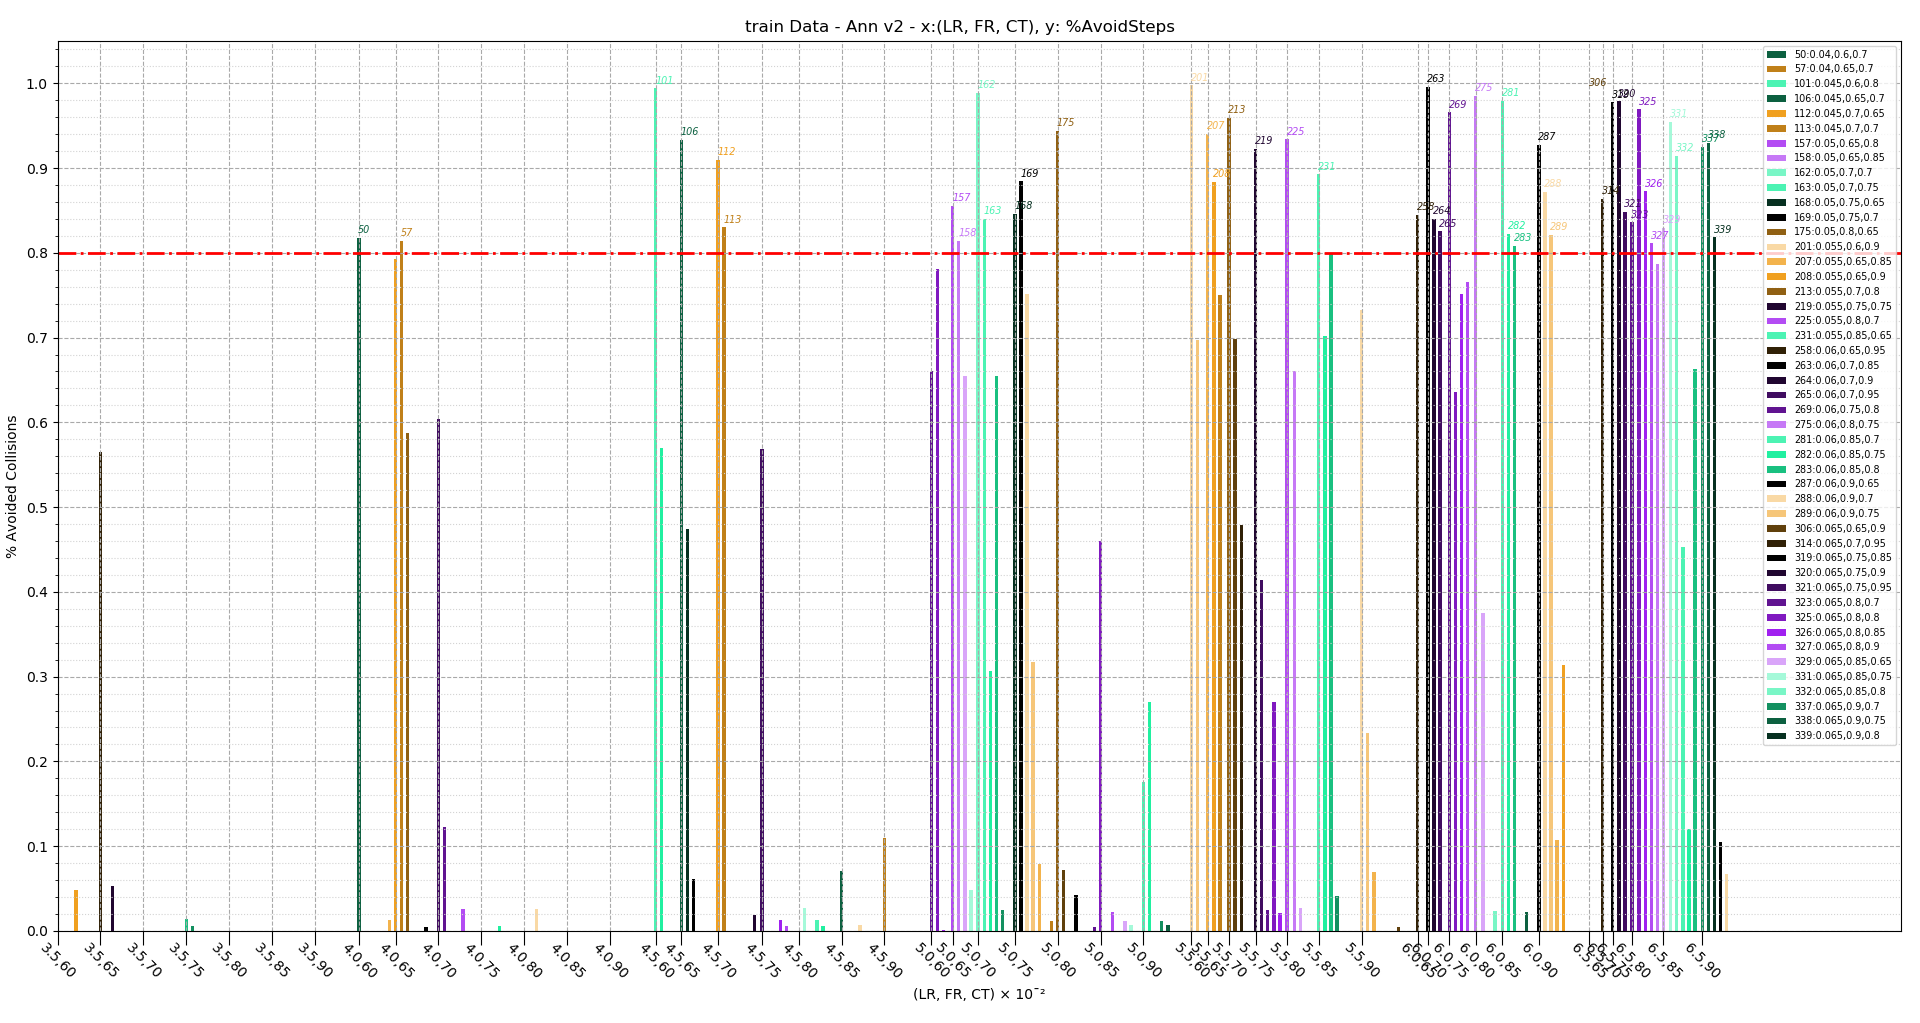
\includegraphics[scale=0.55,rotate=-90]{figures/train_annv2_2d.png}
    \caption{}
    \label{fig:TrainV2}
\end{figure}

\newpage
% \restoregeometry
\thispagestyle{empty}
% \newgeometry{top=5mm, bottom=10mm}

\begin{figure}[H]
    \centering
    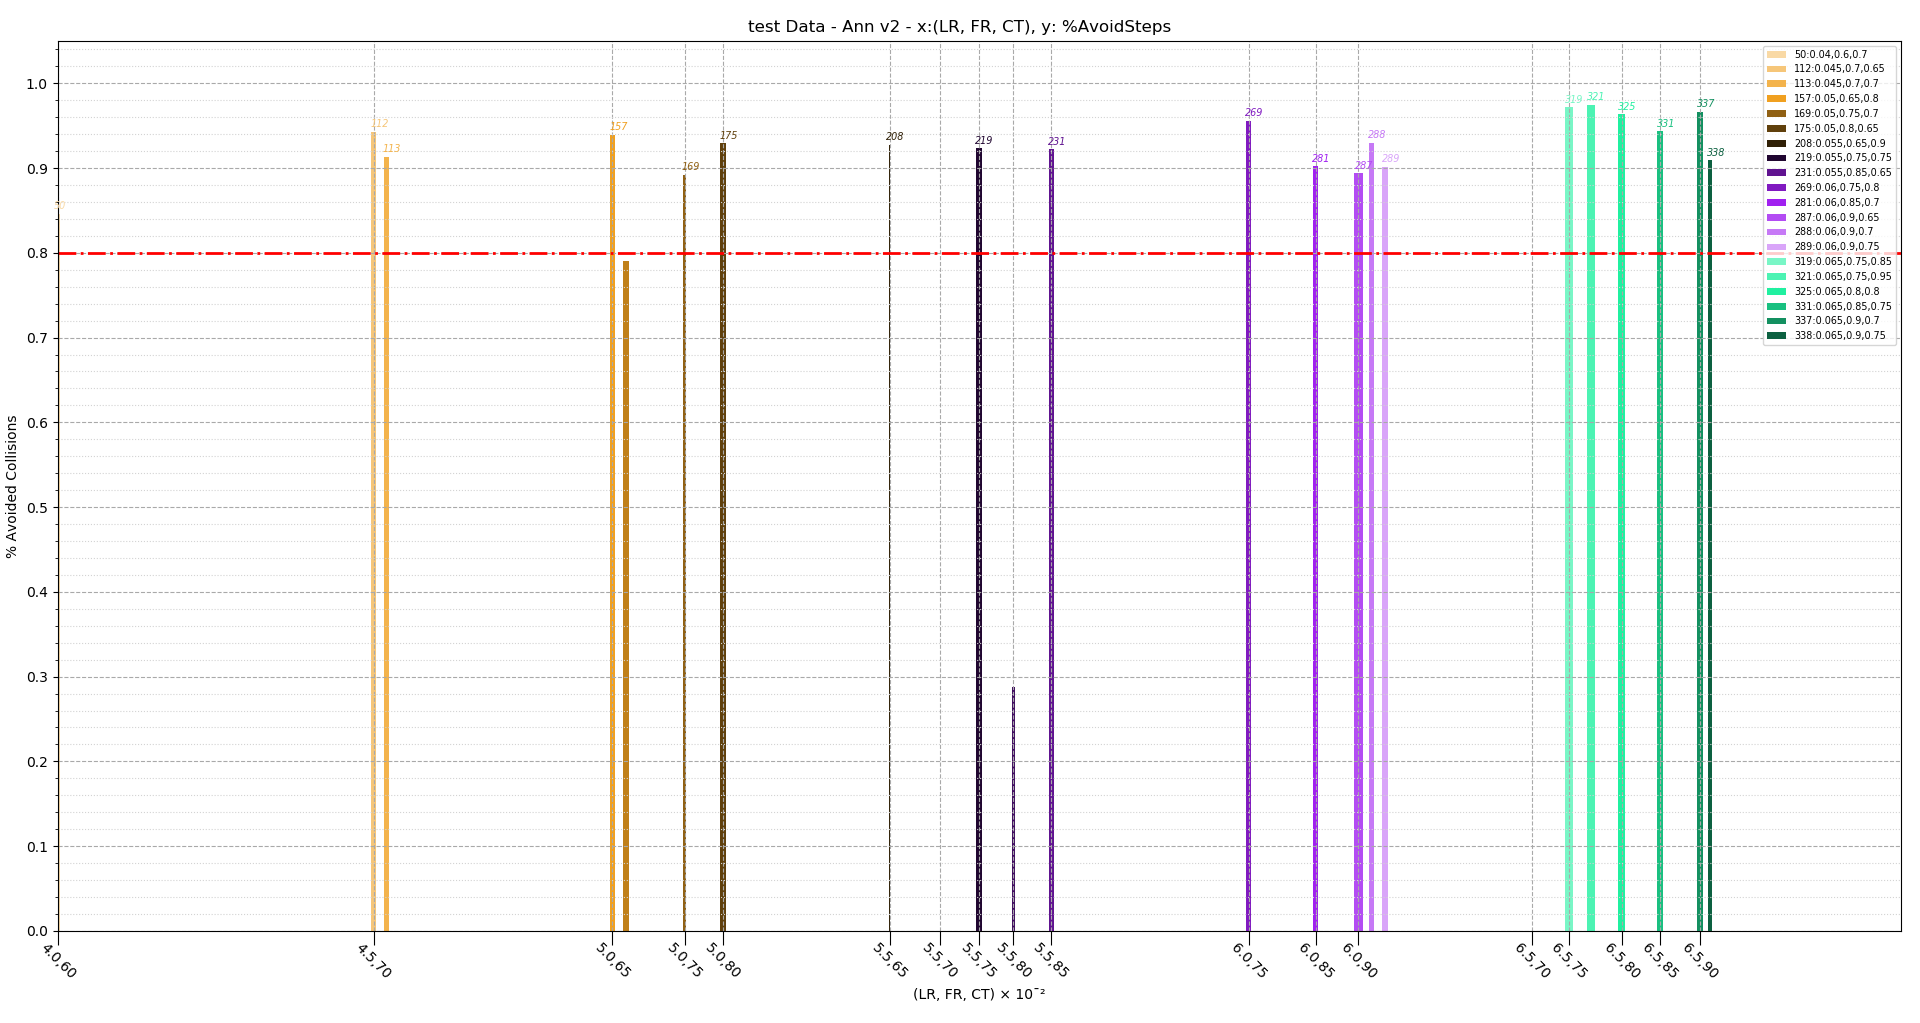
\includegraphics[scale=0.55,rotate=-90]{figures/test_annv2_2d.png}
    \caption{}
    \label{fig:TestV2}
\end{figure}

\newpage
% \restoregeometry
\thispagestyle{empty}
% \newgeometry{top=5mm, bottom=10mm}

\begin{figure}[H]
    \centering
    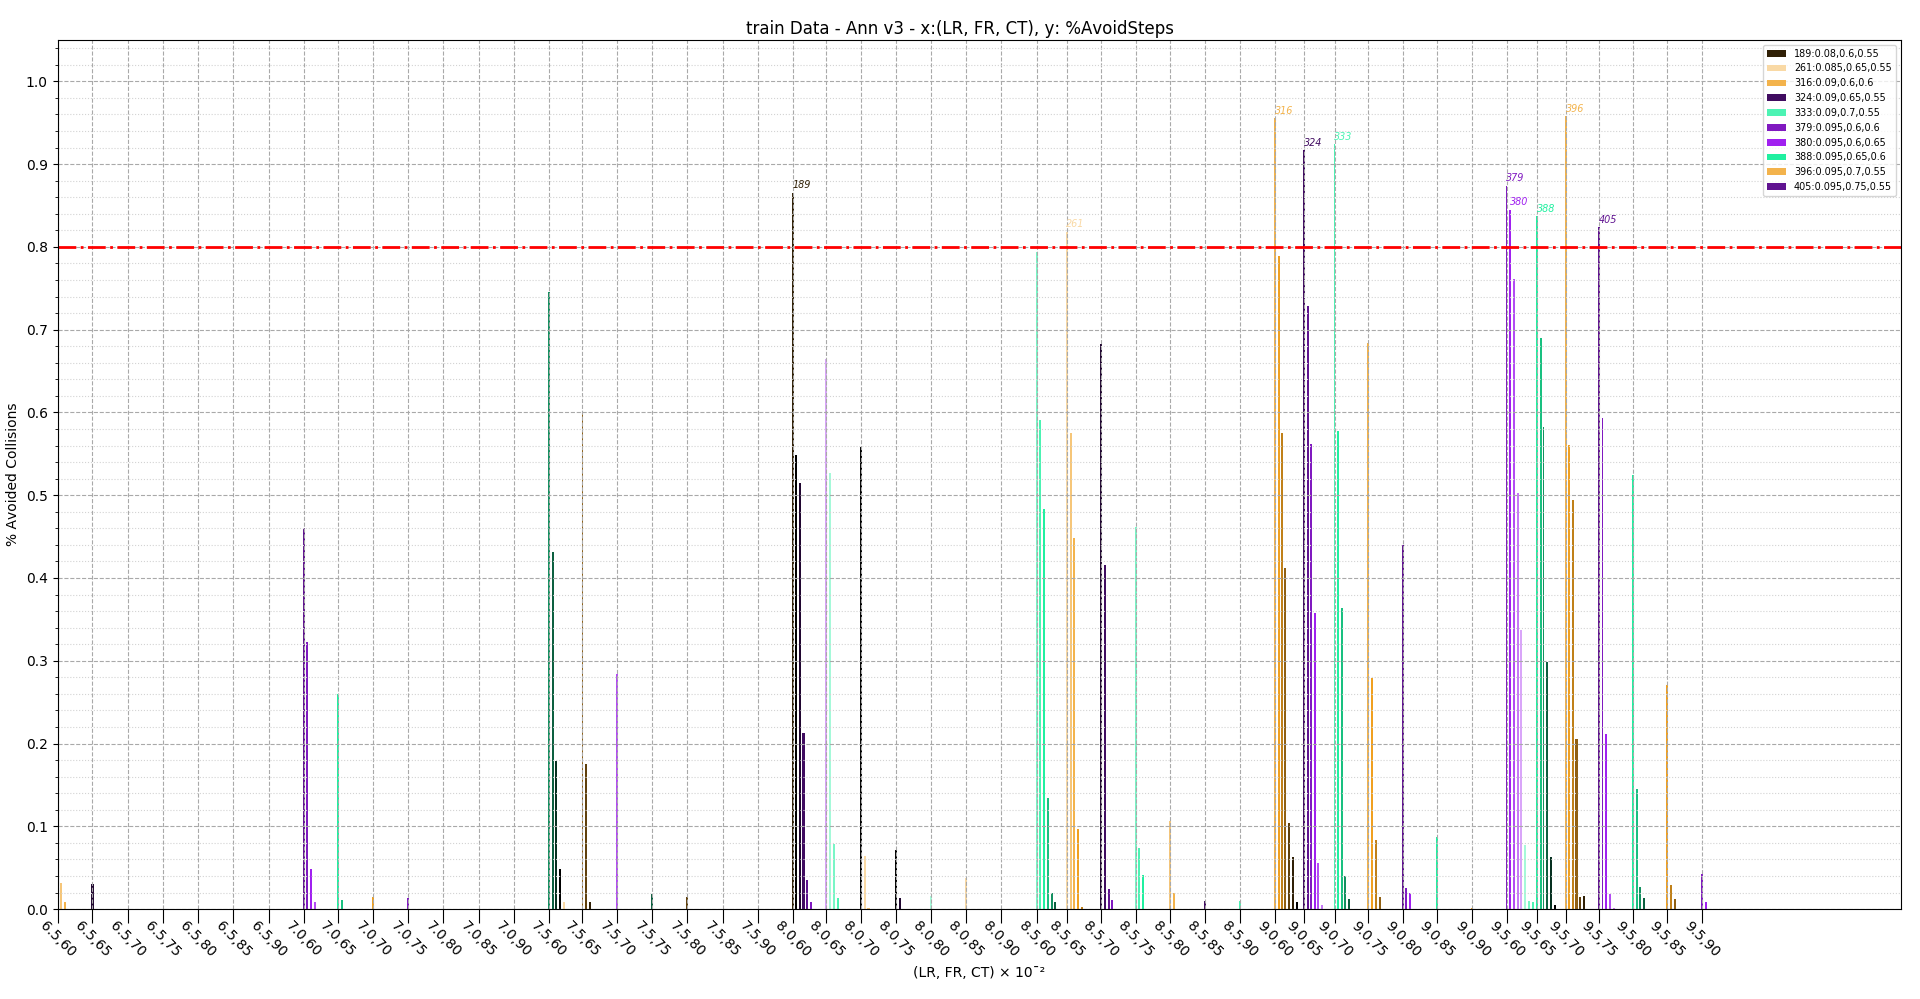
\includegraphics[scale=0.55,rotate=-90]{figures/train_annv3_2d.png}
    \caption{}
    \label{fig:TrainV3}
\end{figure}

\newpage
% \restoregeometry
\thispagestyle{empty}
% \newgeometry{top=5mm, bottom=10mm}

\begin{figure}[H]
    \centering
    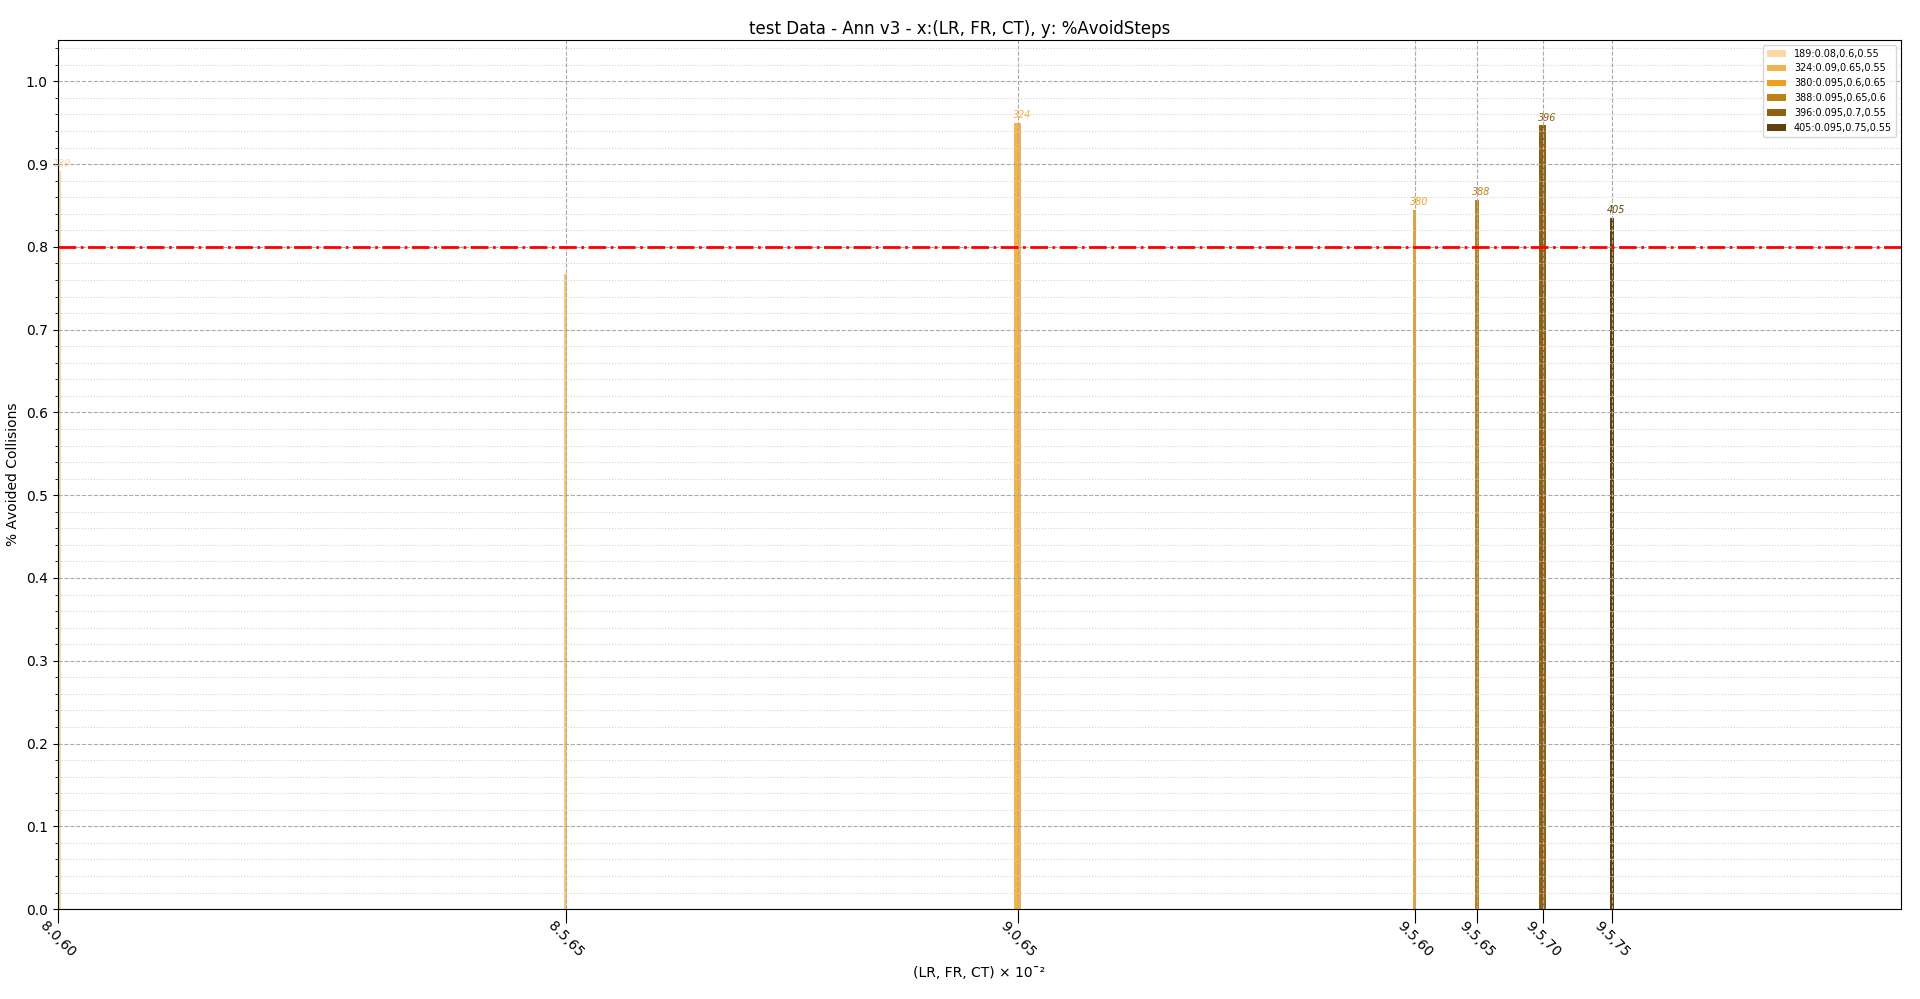
\includegraphics[scale=0.55,rotate=-90]{figures/test_annv3_2d.png}
    \caption{}
    \label{fig:TestV3}
\end{figure}

\newpage
% \restoregeometry
\thispagestyle{empty}
% \newgeometry{top=5mm, bottom=10mm}

\begin{figure}[H]
    \centering
    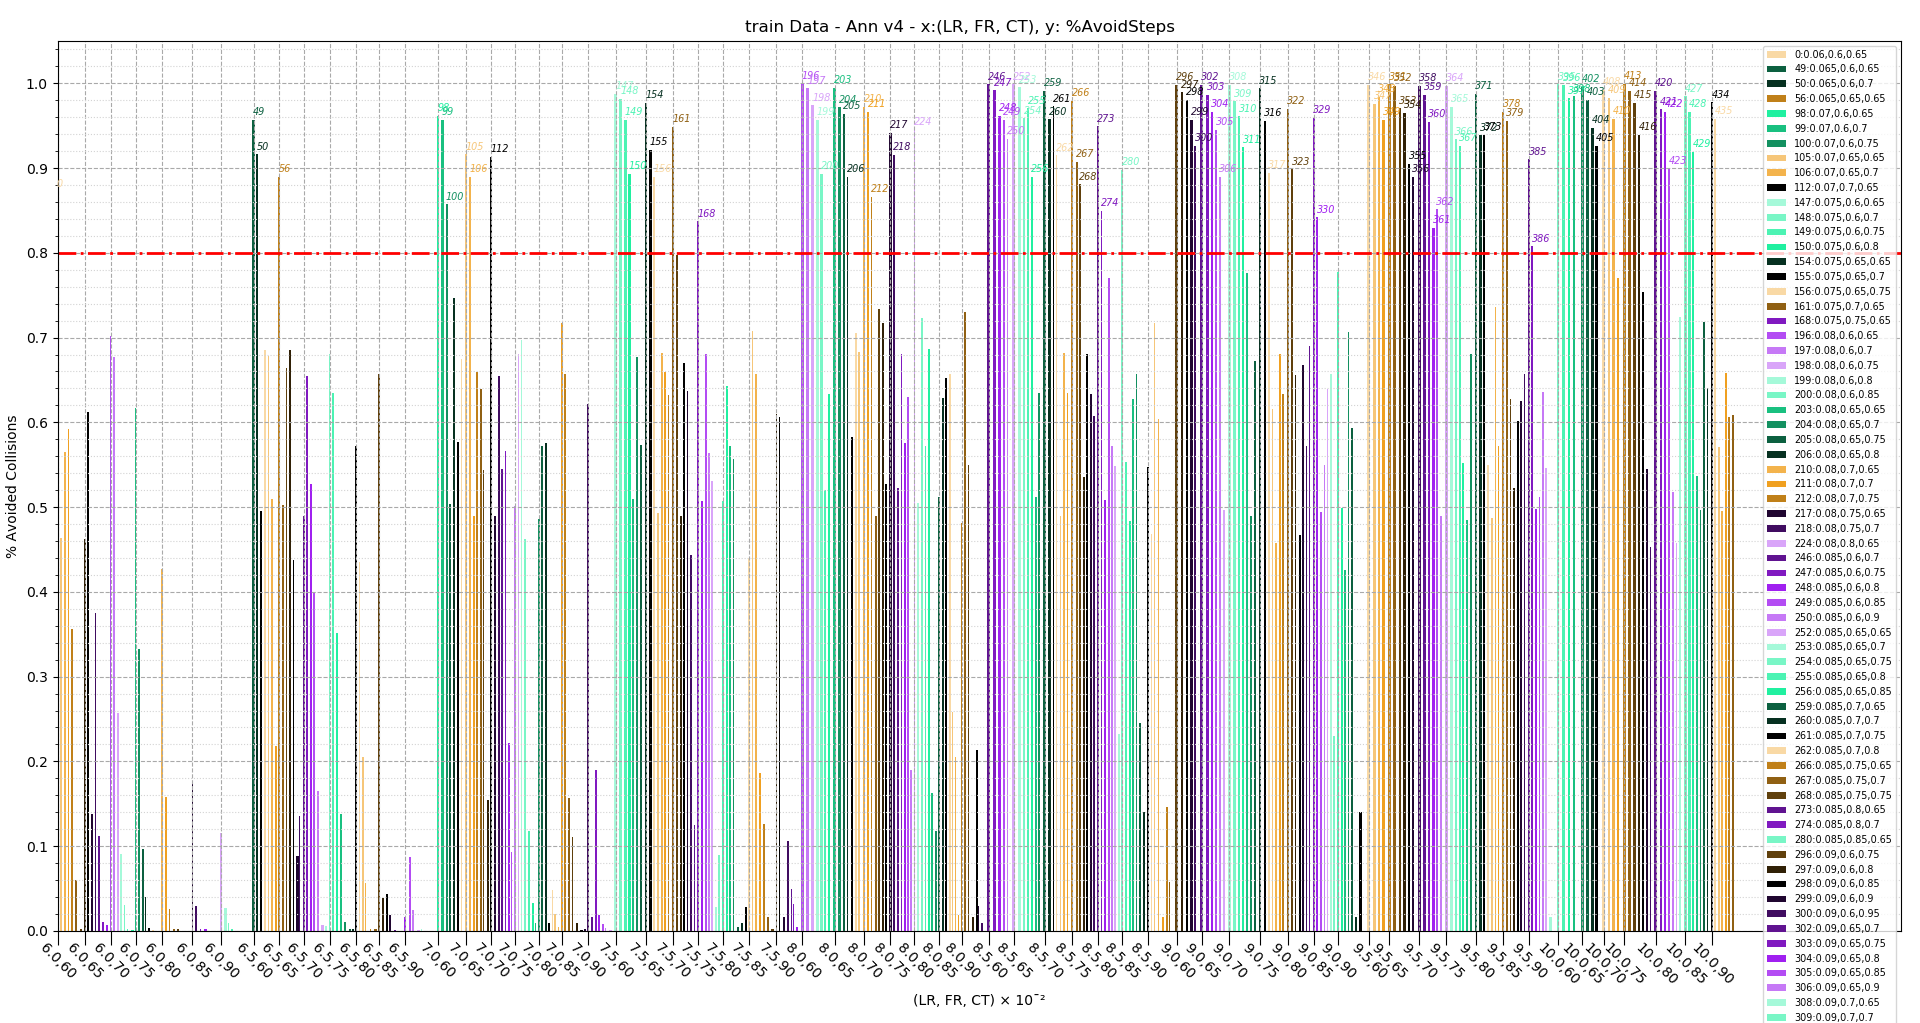
\includegraphics[scale=0.55,rotate=-90]{figures/train_annv4_2d.png}
    \caption{}
    \label{fig:TrainV4}
\end{figure}

\newpage
% \restoregeometry
\thispagestyle{empty}
% \newgeometry{top=5mm, bottom=10mm}

\begin{figure}[H]
    \centering
    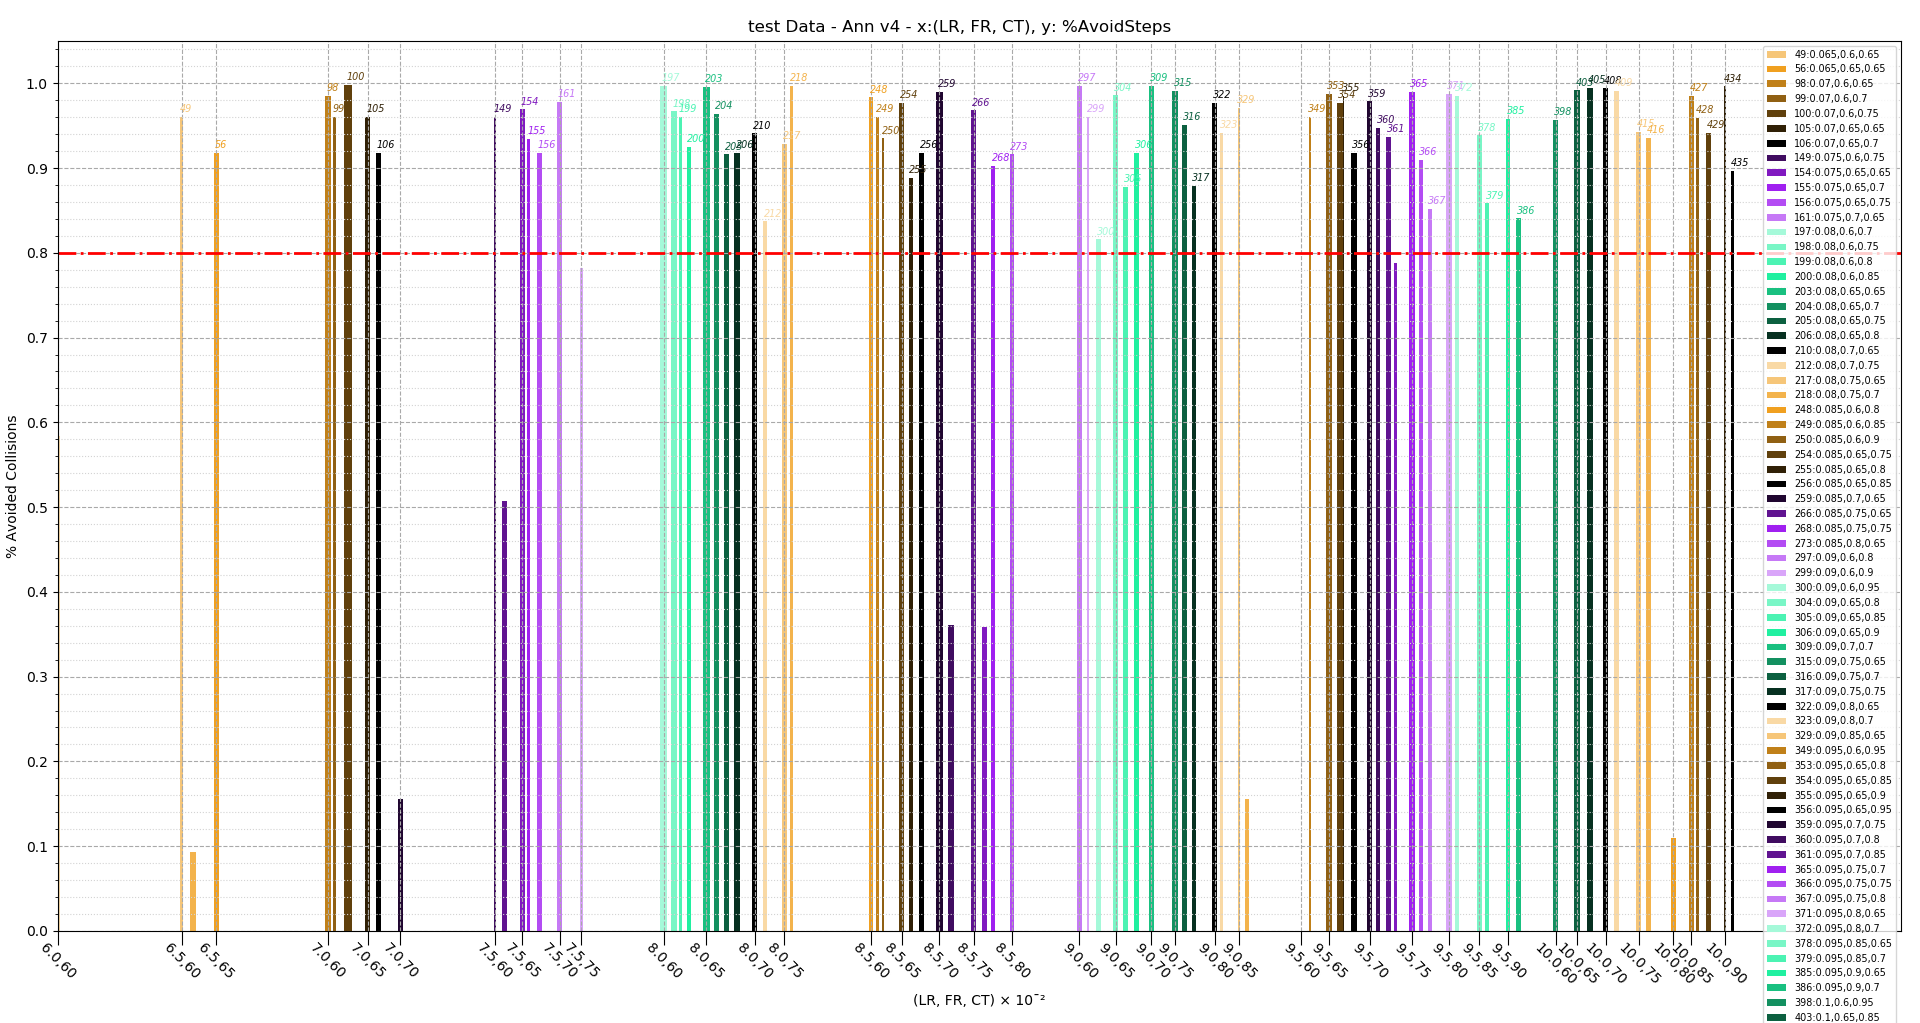
\includegraphics[scale=0.55,rotate=-90]{figures/test_annv4_2d.png}
    \caption{}
    \label{fig:TestV4}
\end{figure}

\newpage
\restoregeometry

% Esponi le problematiche che non si evincono dai dati

\paragraph{Addestramento e Test -- \texttt{dacv2}}\label{par:dacv2}\hfill

Durante gli studi preliminari per individuare una serie di esempi funzionanti attorno alla quale poi ricercare altre possibili configurazioni valide, si è notato un particolare "rapporto" tra i 3 parametri che guidano l'apprendimento: l'incremento di $\eta$ porta ad incrementare $\epsilon$.
Infatti, incrementare $\eta$ senza un adeguato aumento di $\epsilon$ conduce spesso il robot a conseguire un comportamento di tipo circolare. Questo è probabilmente riconducibile alla funzione di apprendimento adoperata che porta la rete ad essere facilmente affetta da \textit{overfitting}: anche per $\eta$ piccoli la rete degenera velocemente, portando il robot a non apprendere. Medesimo discorso vale per $\epsilon$: valori troppo bassi non permettono di compensare la natura saturante di $\eta$ ma, allo stesso tempo, valori eccessivamente elevati senza un adeguato contrasto di $\eta$ portano egualmente all'apprendimento di alcun meccanismo.

Il parametro $\tau_{Collision}$ si comporta in maniera abbastanza variabile rispetto agli altri due parametri ma costituisce un peso fondamentale che fa pendere l'ago della bilancia verso un stato di equilibrio o d'instabilità della rete. 

Questa serie di osservazioni ha portato ad esplorare solo una porzione dello spazio dei parametri per cui $\eta < \epsilon$. Quello che ci si aspettava dunque era di trovare, per ogni \texttt{learning rate} dell'intorno, almeno una coppia di $\epsilon$ e $\tau_{Collision}$ che producesse un modello valido. 

Com'è possibile vedere dai grafici \ref{fig:TrainV2} e \ref{fig:TestV2}, all'incrementare di $\eta$ le aree popolate da modelli "validi" sono in corrispondenza di zone in cui $\epsilon$ è via via leggermente più elevato. Questi poi si diradano quando $\epsilon$ diviene troppo elevato, a causa dell'eccessiva \textit{oscillazione della rete}. É inoltre interessante osservare come il numero di modelli "\textit{validi}" aumenta all'aumentare di $\eta$. Questo può essere riportato alle seguenti possibili motivazioni: 

\begin{enumerate}
    \item il tempo di addestramento (2h) per $\eta$ piccoli é troppo basso 
    \item $\epsilon$ per $\eta$ piccoli è troppo alta
    \item $\tau_{Collision}$ per $\eta$ piccoli è troppo alta
    \item la funzione di apprendimento utilizzata, in congiunzione al modello della rete neurale adoperata, raggiunge un effettivo equilibrio solo per valori elevati dei parametri
\end{enumerate} 

Una problematica dovuta alla presenza di questi parametri particolarmente sbilanciati è che, possedendo $\epsilon$ particolarmente grande, malgrado molti agenti apprendano velocemente il comportamento voluto, questi lo dimentichino anche altrettanto velocemente alla prima nuova collisione. Specialmente con un tempo di addestramento molto elevato, è avvenuto diverse volte che il robot imparasse ad evitare gli ostacoli modestamente ma il lavoro risultasse vanificato a causa di una collisione verso la conclusione del tempo di addestramento oppure perché l'agente si incastrasse in uno degli angoli concavi formati dagli ostacoli dell'arena.

Sebbene non sia stato esplorato completamente lo spazio dei parametri e dunque non siano state addestrate tutte le possibili configurazioni del modello, è evidente che se per valori così bassi di $\eta$ sono necessari valori particolarmente elevati di $\epsilon$ allora il restante spazio di ricerca, individuato \textit{incrementando} tali parametri, difficilmente può contenere ulteriori risultati significativi.
Altri scenari d'interesse esplorabili potrebbero essere quelli per cui $\eta < 0.035$ e $\epsilon < 0.65$, incrementando leggermente (verso il basso) il range dei valori di $\tau_{Collision}$ da esplorare.

Una caratteristica che si è notata in tutti gli agenti di \texttt{dacv2} che apprendono il comportamento desiderato di \textit{Obstacle-Avoidance} è quella di favorire uno specifico lato per evitare "correttamente"\footnote{Come ci aspetteremmo che l'agente eviti l'ostacolo.} gli ostacoli mentro sull'altro lato eseguono una piroetta prima di allontanarsi. Quest'ultimo comportamento "emergente" è, la maggior parte delle volte, la causa delle collisioni che il robot compie durante i suoi periodi di addestramento e test, sebbene questi abbia appreso la corretta associazione tra stimoli e risposte.

Questo comportamento "emergente", unito alla problematica precedentemente descritta, è una delle motivazioni per cui alcuni addestramenti producono un tipo di Falso Positivo particolarmente insidioso: comportamento circolare \textit{non su se stesso} (disegnando una serie di spirali) ma che dimostra egualmente \textit{Obstacle-Avoidance}. Questo particolare modello viene generato quando l'agente giunge vicino ad uno degli angoli concavi dell'arena con il lato che presenta il comportamento "emergente" rivolto verso gli ostacoli. Se questo genere di configurazione si presenta durante la fase di training, porta l'agente ad incastrarsi in un loop di piroette cercando di schivare ambedue gli ostacoli che compongono l'angolo; in fase di test ciò costringe invece l'agente a conseguire una traiettoria curvilinea e dunque presentare il comportamento "spiraliforme" sopra descritto.

A differenza degli altri Falsi Posiviti, dove la traiettoria circolare "in-place" è dovuta alla presenza di una serie di attivazioni costanti nel layer di Collisione, in questo caso il genere di traiettoria è provocata da una serie di \textit{attivazioni sporadiche}\footnote{Ovvero attivazioni non dovute ne ad una collisione ne alla presenza di ostacoli nelle vicinanze.} dei neuroni nel layer di Collisione che inducono il robot a sterzare quando non richiesto. Queste \textit{attivazioni sporadiche} posso essere ricondotte ad oscillazioni del modello della rete neurale appreso e dovute sia ai parametri di apprendimento particolarmente sbilanciati, sia all'interruzione dell'addestramento in una fase di apprendimento (modifica) dei pesi della rete. 

In entrambi i casi di Falsi Positivi, il loro comportamento può essere visto come una sorta di \textit{phantom pain} dell'agente e riportato al medesimo meccanismo: avendo troncato prematuramente l'apprendimento e dunque congelato il modello della rete neurale in una fase di disequilibrio, l'agente è attratto naturalmente ad eseguire più frequentemente l'ultima azione\footnote{Visto come pattern di attivazione dei neuroni nel layer di collisione} effettuata prima dell'arresto.

Per quanto riguarda in generale le prestazioni presentate nei grafici \ref{fig:TrainV2} e \ref{fig:TestV2}, è possibile osservare che le prestazioni migliori si ottengono per $\eta=0.065$ ma mostrando in generale valori inferiori rispetto agli score riportati in fase di addestramento. Al contrario, molti modelli che superano l'addestramento in maniera particolarmente brillante vengono identificati come Falsi Positivi durante i test, probabilmente a causa di una collisione prima della conclusione dell'addestramento.

\newpage

\paragraph{Addestramento e Test -- \textsc{dacv3}} \label{par:dacv3}\hfill

Per quanto riguarda il testing della versione \textit{dacv3} si è partiti prima di tutto ad effettuare un training e testing sfruttando gli stessi intervalli di parametri usati nella \textit{dacv2}. 

Purtroppo però, sia a livello qualitativo osservando il comportamento dell'agente che valutando quantitativamente i grafici, si è notato che tali configurazione fornivano risultati pessimi e in nessun caso riuscivano a portare l'agente ad apprendere. 
Si è quindi proceduto, come effettuato prima del training della \textit{dacv2}, ad una esplorazione empirica del possibile intervallo di valori dei parametri, il quale mostrasse una qualche forma di apprendimento di un comportamento corretto. A parità di \textit{forget rate} si è notato che l'agente cominciava a mostrare segni di apprendimento per valori di \textit{learning rate} maggiori di 0.65 e \textit{collision threshold} a partire da 0.55. 

È stato quindi effettuato un training in batch con intervallo di \textit{learning rate} tra 0.65 e 0.95 e \textit{collision threshold} tra 0.55 e 0.95. Successivamente sono stati selezionati i modelli che in fase di train presentavano una $\texttt{\%AvoidSteps} > 0.8$ per poi effettuare il test su essi.
Rispetto al modello \textit{dacv2} i modelli ottenuti, che presentano comportamenti di apprendimento significativi sono in numero minore, ma allo stesso tempo nessuno di quelli mostrati nel grafico relativo ai test (figura \ref{fig:TestV3}) è un falso positivo.

Osservando i grafici di train (figura \ref{fig:TrainV3}) si può notare che a parità di \textit{learning rate} e \textit{forget rate} aumentando la collision threshold la \texttt{\%AvoidSteps} tende a diminuire sensibilmente e i risultati migliori si ottengono per i valori tra 0.55 e 0.65. 
Sempre dal grafico \ref{fig:TrainV3} si evince che i valori più significativi si ottengono con valori di \textit{learning rate} a partire da 0.08 e si nota anche come all'aumentare del \textit{learning rate} la variazione della \textit{forget rate} e della \textit{collision-threshold} infici di meno sul valore di \texttt{\%AvoidSteps}.

Interessante risulta anche notare come sia in \ref{fig:TrainV3} che in \ref{fig:TestV3} per le coppie di valori [LR=0.09, FR=0.65] e [LR=0.95, FR=0.70] otteniamo dei valori di \texttt{\%AvoidSteps} molto simile.

Considerando che 0.55 è il valore minimo dell'intervallo di variazione della \textit{collision threshold} e considerando che alcuni risultati buoni sono stati ottenuti con tale valore, è stato interessante effettuare un'ulteriore run di training e test esplorando come intervallo il range [0.45,0.65]. Ciò è stato fatto con l'obiettivo di capire se al di sotto di 0.55 potevano essere presenti ulteriori valori interessanti. In questo caso si è scelto di concentrarsi su un intervallo di \textit{learning rate} contenenti i valori significativi ottenuti nella run mostrata nei grafici. Per la precisione $LR \in [0.085, 0.095]$. Mentre per quanto riguarda la FR è stato scelto il valore 0.6.
Ciò ha mostrato solo valori nulli di \texttt{\%AvoidSteps} al di sotto di una \textit{collision threshold} di 0.55.

Analizzando invece il comportamento a livello qualitativo, anche per quanto riguarda la versione \textit{dacv3} notiamo che l'agente apprende correttamente quando schivare gli ostacoli, ma effettuando schivate sempre verso destra, che nel caso in cui l'ostacolo si trovi da quella parte porta il robot ad effettuare una piroetta. Ciò è dovuto molto probabilmente alle stesse ragioni precedentemente esposte. 

Ricordando che la struttura della rete \textit{dacv3} è stata fatta sulla base della struttura descritta nel paper \cite{verschure1992distributed} e osservando il range di valori in cui abbiamo risultati migliori, si può notare che esso si avvicina ai valori dei parametri di apprendimento usati dagli autori del paper. Ciò può essere interpretato sia come una parziale conferma all'attendibilità dei valori riportati nel paper, sia come una corretta interpretazione da parte nostra del modello, nonostante l'assenza di alcuni elementi chiave. 

\newpage

\paragraph{Addestramento e Test -- \texttt{dacv4}}\label{par:dacv4}\hfill

Come già detto in fase di progettazione, \texttt{dacv4} nasce dal modello di \texttt{dacv2} al fine di comprendere come il comportamento e l'apprendimento di quest'ultima fosse influenzato dal numero di sensori, e dunque di neuroni, effettivamente utilizzati dall'agente. In tal senso questo modello si dimostra particolarmente interessante:

\begin{itemize}
    \item Da una parte il comportamento esterno dell'agente si è presentato non essere affatto dissimile da quello espresso utilizzando il modello di \texttt{dacv2}. Infatti, come per \texttt{dacv2}, il robot presenta i medesimi "pattern" di schivate: apprende "correttamente" a schivare l'ostacolo da un certo lato, ma per l'altro esegue una piroetta prima di allontanarsi. Questo lo porta a dimostrare anche le medesime problematiche presentate per \texttt{dacv2} e \texttt{dacv3}.
    
    \item Dall'altra, è qui risiede la fondamentale differenza dei due modelli, il quantitativo di modelli che risultano validi è cresciuto enormemente, attestandosi anche score particolarmente elevati. Malgrado non sia mostrato nei grafici, l'addestramento di \texttt{dacv4} nel medesimo spazio di parametri di \texttt{dacv2} ha prodotto solo qualche modello interessante per $\eta \ge 0.06$. Spostando l'addestramento verso parametri di apprendimento più elevati, $\eta \in [0.06, 0.1]$, il numero di modelli "validi" è incrementato esponenzialmente.
    
    Questo indica che il modello \texttt{dacv4} raggiunge l'equilibrio con valori di $\eta$ maggiori a parità dei medesimi spazi di ricerca per $\epsilon$ e $\tau$, portandosi leggermente più vicino ai valori di apprendimento riportati nel paper \cite{verschure1992distributed}. D'altro canto però tale risultato si pone come arma a doppio taglio in quanto è necessariamente sintomo di una maggiore probabilità di Falsi Positivi del secondo tipo (vedi \ref{par:dacv2}).
\end{itemize}

A differenza di \texttt{dacv2} le prestazioni in questo caso si dimostrano maggiormente constanti al variare dei parametri di apprendimento e decisamente più alte, sebbene alcuni dei modelli migliori come \texttt{100}, \texttt{197} e \texttt{297} risultano essere dei Falsi Positivi del secondo tipo.  


